\documentclass[preview,border=0mm,convert={convertexe={magick},outext=.ps}]{standalone}
\usepackage[dvipdfm]{geometry}
%graphics
\usepackage{xcolor}
\usepackage{tikz}
\usetikzlibrary{external,calc,math,arrows.meta,intersections,backgrounds}
\usepackage[caption=false,font=footnotesize]{subfig}

%from Torres
% \definecolor{clock0}{HTML}{008000}
% \definecolor{clock1}{HTML}{800080}
% \definecolor{clock2}{HTML}{008080}
% \definecolor{clock3}{HTML}{F2F2F2}
% \definecolor{input}{HTML}{3663B2}
% \definecolor{output}{HTML}{D47000}
% \definecolor{fixed}{HTML}{000000}
%from fiction
\definecolor{clock1}{HTML}{86E291}
\definecolor{clock2}{HTML}{FFA5FA}
\definecolor{clock3}{HTML}{00C8BC}
\definecolor{clock4}{HTML}{F2F2F2}
\definecolor{input}{HTML}{008DC8}
\definecolor{output}{HTML}{E28686}
\definecolor{fixed}{HTML}{000000}
%colorful
% \definecolor{clock0}{RGB}{68, 189, 50}
% \definecolor{clock1}{RGB}{140, 122, 230}
% \definecolor{clock2}{RGB}{0, 151, 230}
% \definecolor{clock3}{RGB}{192,192,192}
% \definecolor{input}{RGB}{39, 60, 117}
% \definecolor{output}{RGB}{255,159,67}
% \definecolor{fixed}{RGB}{20,20,20}
%\definecolor{output}{RGB}{255,242,0}
%\definecolor{fixed}{RGB}{255, 159, 67}
%dark color
% \definecolor{clock0}{RGB}{0,150,136}
% \definecolor{clock1}{RGB}{123,104,238}
% \definecolor{clock2}{RGB}{135,206,250}
% \definecolor{clock3}{RGB}{128,128,128}
% \definecolor{input}{RGB}{65,105,225}
% \definecolor{output}{RGB}{255,165,0}
% \definecolor{fixed}{RGB}{32,32,32}
%light color
% \definecolor{clock0}{RGB}{153,204,51}
% \definecolor{clock1}{RGB}{204,204,255}
% \definecolor{clock2}{RGB}{122,224,255}
% \definecolor{clock3}{RGB}{204,204,204}
% \definecolor{input}{RGB}{153,204,255}
% \definecolor{output}{RGB}{255,204,153}
% \definecolor{fixed}{RGB}{110,110,110}

\colorlet{dot-color}{black!80}
\colorlet{cs1}{lightgray!20}
\colorlet{cs2}{lightgray!50}
\colorlet{cs3}{lightgray}
\colorlet{cs4}{gray}
\def\cellsize{0.425}
\tikzset{
  pics/gcell/.style = {
    code = {
      \coordinate (-center) at (0,0);
      
      \fill +(-0.45,-0.45) coordinate(-sw) 
      -- +(-0.45, 0.45) coordinate(-nw)
      -- +( 0.45, 0.45) coordinate(-ne)
      -- +( 0.45,-0.45) coordinate(-se)
      -- cycle;
      \coordinate (-swo) at ($ (-center)!0.5!(-sw) $);
      \coordinate (-nwo) at ($ (-center)!0.5!(-nw) $);
      \coordinate (-neo) at ($ (-center)!0.5!(-ne) $);
      \coordinate (-seo) at ($ (-center)!0.5!(-se) $);
      
      \coordinate (-south) at ($ (-sw)!.5!(-se) $);
      \coordinate (-north) at ($ (-nw)!.5!(-ne) $);
      \coordinate (-west)  at ($ (-sw)!.5!(-nw) $);
      \coordinate (-east)  at ($ (-se)!.5!(-ne) $);
      
      \fill[white] (-swo) let \p1=($ (-center)!.5!(-swo) $) in circle ({veclen(\x1,\y1)});
      \fill[white] (-nwo) let \p1=($ (-center)!.5!(-nwo) $) in circle ({veclen(\x1,\y1)});
      \fill[white] (-neo) let \p1=($ (-center)!.5!(-neo) $) in circle ({veclen(\x1,\y1)});
      \fill[white] (-seo) let \p1=($ (-center)!.5!(-seo) $) in circle ({veclen(\x1,\y1)});
      
      \ifnum#1=1\relax
      \fill[dot-color] (-swo) let \p1=($ (-center)!.32!(-swo) $) in circle ({veclen(\x1,\y1)});
      \fill[dot-color] (-neo) let \p1=($ (-center)!.32!(-neo) $) in circle ({veclen(\x1,\y1)});
      \else
      \ifnum#1=-1\relax
      \fill[dot-color] (-nwo) let \p1=($ (-center)!.32!(-nwo) $) in circle ({veclen(\x1,\y1)});
      \fill[dot-color] (-seo) let \p1=($ (-center)!.32!(-seo) $) in circle ({veclen(\x1,\y1)});
      \else
      \fill[dot-color] (-swo) let \p1=($ (-center)!.22!(-swo) $) in circle ({veclen(\x1,\y1)});
      \fill[dot-color] (-nwo) let \p1=($ (-center)!.22!(-nwo) $) in circle ({veclen(\x1,\y1)});
      \fill[dot-color] (-neo) let \p1=($ (-center)!.22!(-neo) $) in circle ({veclen(\x1,\y1)});
      \fill[dot-color] (-seo) let \p1=($ (-center)!.22!(-seo) $) in circle ({veclen(\x1,\y1)});
      \fi
      \fi
    }
  },
  pics/gcell/.default={0},
  pics/gcross_cell/.style = {
    code = {%
      \coordinate (-center) at (0,0);
      \fill +(-0.45,-0.45) coordinate(-sw) 
      -- +(-0.45, 0.45) coordinate(-nw)
      -- +( 0.45, 0.45) coordinate(-ne)
      -- +( 0.45,-0.45) coordinate(-se)
      -- cycle;
      \coordinate (-north) at ($(-ne)!0.5!(-nw)$);
      \coordinate (-south) at ($(-se)!0.5!(-sw)$);
      \coordinate (-east) at ($(-ne)!0.5!(-se)$);
      \coordinate (-west) at ($(-nw)!0.5!(-sw)$);
      
      \coordinate (-no) at ($(-center)!0.65!(-north)$);
      \coordinate (-so) at ($(-center)!0.65!(-south)$);
      \coordinate (-eo) at ($(-center)!0.65!(-east)$);
      \coordinate (-wo) at ($(-center)!0.65!(-west)$);
      
      \fill[white] (-no) let \p1=($ (-center)!0.5!(-no) $) in circle ({veclen(\x1,\y1)});
      \fill[white] (-so) let \p1=($ (-center)!0.5!(-so) $) in circle ({veclen(\x1,\y1)});
      \fill[white] (-eo) let \p1=($ (-center)!0.5!(-eo) $) in circle ({veclen(\x1,\y1)});
      \fill[white] (-wo) let \p1=($ (-center)!0.5!(-wo) $) in circle ({veclen(\x1,\y1)});
      
      \ifnum#1=1\relax
      \fill[dot-color] (-no) let \p1=($ (-center)!.32!(-no) $) in circle ({veclen(\x1,\y1)});
      \fill[dot-color] (-so) let \p1=($ (-center)!.32!(-so) $) in circle ({veclen(\x1,\y1)});
      \else
      \ifnum#1=-1\relax
      \fill[dot-color] (-eo) let \p1=($ (-center)!.32!(-eo) $) in circle ({veclen(\x1,\y1)});
      \fill[dot-color] (-wo) let \p1=($ (-center)!.32!(-wo) $) in circle ({veclen(\x1,\y1)});
      \fi
      \fi
    }
  },
  pics/cell/.style = {
    code = {%
      \coordinate (-center) at (0,0);
      \coordinate (-east) at (\cellsize, 0);
      \coordinate (-north) at (0, \cellsize);
      \coordinate (-west) at (-\cellsize, 0);
      \coordinate (-south) at (0, -\cellsize);
      
      \fill[draw=black, line width=0.2pt, rounded corners=0.3pt] (-west |- -south) rectangle (-east |- -north);
      \foreach \d in {-east, -north, -west, -south}
      \draw[black, line width=.2pt] ($(-center)!.7!45:(\d)$) circle[radius=.12];
    }
  },
  pics/via/.style={
    code={%
      \coordinate (-center) at (0,0);
      \coordinate (-east) at (\cellsize, 0);
      \coordinate (-north) at (0, \cellsize);
      \coordinate (-west) at (-\cellsize, 0);
      \coordinate (-south) at (0, -\cellsize);
      
      \fill[draw=black, line width=0.2pt, rounded corners=0.3pt] (-west |- -south) rectangle (-east |- -north);
      \draw[black, line width=0.2pt] (-center) circle [radius=0.32];
    }
  },
  pics/crossline/.style={
    code={%
      \coordinate (-center) at (0,0);
      \coordinate (-east) at (\cellsize, 0);
      \coordinate (-north) at (0, \cellsize);
      \coordinate (-west) at (-\cellsize, 0);
      \coordinate (-south) at (0, -\cellsize);
      
      \fill[draw=black, line width=0.2pt, rounded corners=0.3pt] (-west |- -south) rectangle (-east |- -north);
      \foreach \d in {-east, -north, -west, -south}
      \draw[black, line width=.2pt] (-center) -- ($(-center)!.9!45:(\d)$);
    }
  },
  pics/fixed/.style={
    code={%
      \coordinate (-center) at (0,0);
      \coordinate (-east) at (\cellsize, 0);
      \coordinate (-north) at (0, \cellsize);
      \coordinate (-west) at (-\cellsize, 0);
      \coordinate (-south) at (0, -\cellsize);
      
      \fill[draw=black, line width=0.2pt, rounded corners=0.3pt] (-west |- -south) rectangle (-east |- -north);
      \ifnum#1=0\relax
      \foreach \d in {-north, -south}
      \filldraw[white, line width=.2pt] ($(-center)!.7!45:(\d)$) circle[radius=.12];
      \else
      \foreach \d in {-east, -west}
      \filldraw[white, line width=.2pt] ($(-center)!.7!45:(\d)$) circle[radius=.12];
      \fi
    }
  },
}


\begin{document}
 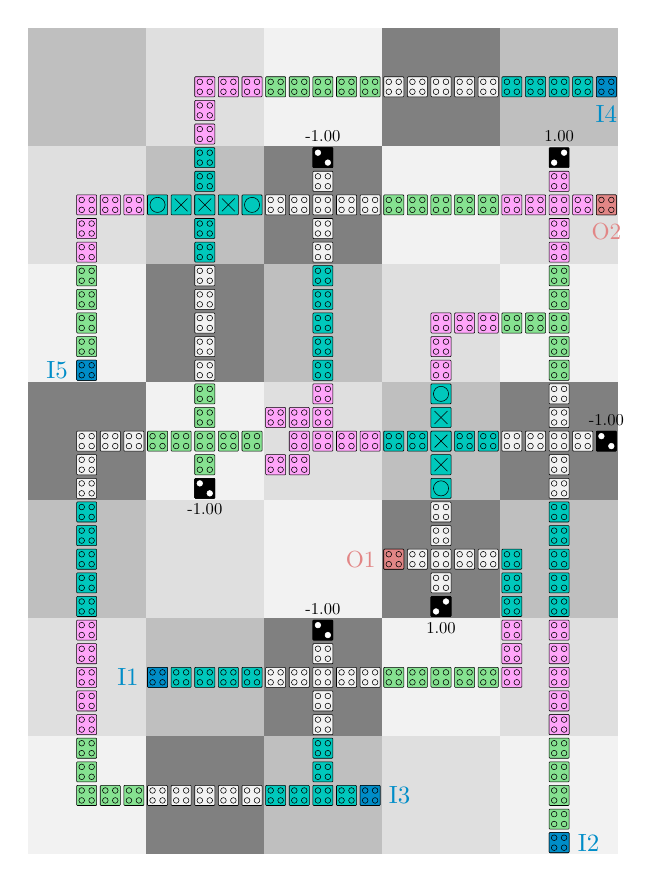
\begin{tikzpicture}[
        xscale=0.3,yscale=0.3
        ]
        \begin{scope}[
          x=5cm,y=5cm,
          shift={(2.5cm,2.5cm)},
          c1/.style={shape=rectangle, fill=cs1, text=black, minimum size=5cm},
          c2/.style={shape=rectangle, fill=cs2, text=black, minimum size=5cm},
          c3/.style={shape=rectangle, fill=cs3, text=black, minimum size=5cm},
          c4/.style={shape=rectangle, fill=cs4, text=black, minimum size=5cm},
          ]
          \tikzmath{
            function use(\x,\y){
              return (mod(\y,2)!=0) ? ((mod(\y+1,4)!=0)?(1+mod(\x+1,4)):(1+mod(\x+3,4))):((mod(\y,4)==0)?(4-mod(\x+3,4)):(4-mod(\x+1,4)));
            };
            %
            int \i, \j, \c; 
            for \i in {0,...,6}{
              for \j in {0,...,4}{
                \c = use(\j,\i);
                {
                  \path (\j,\i)
                  {[transform shape]node(\j\i)[c\c]{}};
%                   ($(\i\j.center)!.8!(\i\j.north east)$) node{};
                };
              };
            };
          }
        \end{scope}
        
        \begin{scope}[
          shift={(0.4975cm,0.4975cm)},
          ]
          \begin{scope}[transform shape]
            \path
            % I1
            (5,7)   pic   [input]{cell}             
            (6,7)   pic   [clock3]{cell}             
            (7,7)   pic   [clock3]{cell} 
            (8,7)   pic   [clock3]{cell}
            (9,7)   pic   [clock3]{cell}
            % node 6
            (10,7)  pic   [clock4]{cell}             
            (11,7)  pic   [clock4]{cell} 
            (12,7)  pic   [clock4]{cell}             
            (13,7)  pic   [clock4]{cell}
            (14,7)  pic   [clock4]{cell}
            (12,5)  pic   [clock4]{cell}               
            (12,6)  pic   [clock4]{cell}             
            (12,8)  pic   [clock4]{cell}
            (12,9)  pic   [fixed]{fixed=0}
            ;
            \path
            (15,7)  pic   [clock1]{cell} 
            (16,7)  pic   [clock1]{cell}               
            (17,7)  pic   [clock1]{cell}               
            (18,7)  pic   [clock1]{cell}
            (19,7)  pic   [clock1]{cell}  
            
            (20,7)  pic   [clock2]{cell}             
            (20,8)  pic   [clock2]{cell}
            (20,9)  pic   [clock2]{cell}               
            ;
            \path
            % I3
            (14,2)  pic   [input]{cell}
            (13,2)  pic   [clock3]{cell}
            (12,2)  pic   [clock3]{cell}
            (12,3)  pic   [clock3]{cell}
            (12,4)  pic   [clock3]{cell}
            (11,2)  pic   [clock3]{cell}
            (10,2)  pic   [clock3]{cell}
            ; 
            \path
            (9,2)  pic   [clock4]{cell}
            (8,2)  pic   [clock4]{cell}
            (7,2)  pic   [clock4]{cell}               
            (6,2)  pic   [clock4]{cell}             
            (5,2)  pic   [clock4]{cell}
            
            (4,2)  pic   [clock1]{cell} 
            (3,2)  pic   [clock1]{cell}               
            (2,2)  pic   [clock1]{cell}               
            (2,3)  pic   [clock1]{cell}
            (2,4)  pic   [clock1]{cell} 
            
            (2,5)  pic   [clock2]{cell} 
            (2,6)  pic   [clock2]{cell} 
            (2,7)  pic   [clock2]{cell} 
            (2,8)  pic   [clock2]{cell}             
            (2,9)  pic   [clock2]{cell}             
            
            (2,10)  pic   [clock3]{cell} 
            (2,11)  pic   [clock3]{cell} 
            (2,12)  pic   [clock3]{cell} 
            (2,13)  pic   [clock3]{cell}             
            (2,14)  pic   [clock3]{cell} 
            
            (2,15)  pic   [clock4]{cell} 
            (2,16)  pic   [clock4]{cell} 
            (2,17)  pic   [clock4]{cell} 
            (3,17)  pic   [clock4]{cell}             
            (4,17)  pic   [clock4]{cell}
            ;
            \path
            % node 7
            (5,17)  pic   [clock1]{cell} 
            (6,17)  pic   [clock1]{cell} 
            (7,17)  pic   [clock1]{cell} 
%             (8,18)  pic   [clock1]{cell} 
            (8,17)  pic   [clock1]{cell}             
            (9,17)  pic   [clock1]{cell}
%             (8,16)  pic   [clock1]{cell}            
            (7,18)  pic   [clock1]{cell} 
            (7,19)  pic   [clock1]{cell}
            ;
            
            \path
            % I4- ndoe 7
            (24,32)  pic   [input]{cell}            
            (23,32)  pic   [clock3]{cell} 
            (22,32)  pic   [clock3]{cell} 
            (21,32)  pic   [clock3]{cell}
            (20,32)  pic   [clock3]{cell}
            
            (19,32)  pic   [clock4]{cell}
            (18,32)  pic   [clock4]{cell} 
            (17,32)  pic   [clock4]{cell}
            (16,32)  pic   [clock4]{cell}
            (15,32)  pic   [clock4]{cell}
            
            (14,32)  pic   [clock1]{cell}
            (13,32)  pic   [clock1]{cell}
            (12,32)  pic   [clock1]{cell}
            (11,32)  pic   [clock1]{cell}
            (10,32)  pic   [clock1]{cell}

            (9,32)   pic   [clock2]{cell}
            (8,32)   pic   [clock2]{cell}
            (7,32)   pic   [clock2]{cell}
            (7,31)   pic   [clock2]{cell}
            (7,30)   pic   [clock2]{cell}            

            (7,29)   pic   [clock3]{cell}
            (7,28)   pic   [clock3]{cell}
            (7,27)   pic   [clock3]{cell}
            (7,26)   pic   [clock3]{cell}
            (7,25)   pic   [clock3]{cell}  

            (7,24)   pic   [clock4]{cell}
            (7,23)   pic   [clock4]{cell}
            (7,22)   pic   [clock4]{cell}
            (7,21)   pic   [clock4]{cell}
            (7,20)   pic   [clock4]{cell}  
            % node 7
            (7,16)   pic    [clock1]{cell}
            (7,15)   pic    [fixed]{fixed=0}
            ;
            \path 
            % I2 - node 8 node 9
            (22,0)  pic   [input]{cell}            
            (22,1)  pic   [clock1]{cell}            
            (22,2)  pic   [clock1]{cell}  
            (22,3)  pic   [clock1]{cell}              
            (22,4)  pic   [clock1]{cell}              
            (22,5)  pic   [clock1]{cell}  
            
            (22,5)  pic   [clock2]{cell}              
            (22,6)  pic   [clock2]{cell}              
            (22,7)  pic   [clock2]{cell}              
            (22,8)  pic   [clock2]{cell}              
            (22,9)  pic   [clock2]{cell} 
            
            (22,10) pic   [clock3]{cell}            
            (22,11) pic   [clock3]{cell}            
            (22,12) pic   [clock3]{cell}
            (22,13) pic   [clock3]{cell}
            (22,14) pic   [clock3]{cell} 
            
            (22,15) pic   [clock4]{cell}            
            (22,16) pic   [clock4]{cell}            
            (22,17) pic   [clock4]{cell}            
            (22,18) pic   [clock4]{cell}
            (22,19) pic   [clock4]{cell}
           % node 8 
            (21,17) pic   [clock4]{cell}
            (20,17) pic   [clock4]{cell}
            (23,17) pic   [clock4]{cell}
            (24,17) pic   [fixed]{fixed=0}
            ;
            \path
           % node 7- node 8
            (11,18) pic   [clock2]{cell}  
            (10,18) pic   [clock2]{cell} 
            (10,16) pic   [clock2]{cell}
            (11,16) pic   [clock2]{cell}             
            (11,17) pic   [clock2]{cell}
            (12,17) pic   [clock2]{cell}  
            (13,17) pic   [clock2]{cell}            
            (14,17) pic   [clock2]{cell} 
            
            (15,17) pic   [clock3]{cell}             
            (16,17) pic   [clock3]{cell}             
            (17,17) pic   [clock3]{cell}
            (18,17) pic   [clock3]{cell}
            (19,17) pic   [clock3]{cell} 
          
            ;
            \path
%             node 7 - node 10            
            (12,18) pic   [clock2]{cell}             
            (12,19) pic   [clock2]{cell}
            
            (12,20) pic   [clock3]{cell}             
            (12,21) pic   [clock3]{cell}            
            (12,22) pic   [clock3]{cell}             
            (12,23) pic   [clock3]{cell}              
            (12,24) pic   [clock3]{cell}
            
            (10,27) pic   [clock4]{cell}
            (11,27) pic   [clock4]{cell}
            (12,27) pic   [clock4]{cell}
            (13,27) pic   [clock4]{cell}
            (14,27) pic   [clock4]{cell}
            (12,28) pic   [clock4]{cell}            
            (12,26) pic   [clock4]{cell}            
            (12,25) pic   [clock4]{cell}
            (12,29) pic   [fixed]{fixed=0}            
            ;
            \path
            % node 10- node 11
            (15,27) pic   [clock1]{cell}
            (16,27) pic   [clock1]{cell}
            (17,27) pic   [clock1]{cell}            
            (18,27) pic   [clock1]{cell}
            (19,27) pic   [clock1]{cell}
            
            (20,27) pic   [clock2]{cell}
            (21,27) pic   [clock2]{cell}            
            (22,27) pic   [clock2]{cell}
            (23,27) pic   [clock2]{cell}
            (24,27) pic   [output]{cell}
            
            (22,26) pic   [clock2]{cell}
            (22,25) pic   [clock2]{cell}
            
            (22,24) pic   [clock1]{cell}
            (22,23) pic   [clock1]{cell}
            (22,22) pic   [clock1]{cell}
            (22,21) pic   [clock1]{cell}
            (22,20) pic   [clock1]{cell}

            (21,22) pic   [clock1]{cell}
            (20,22) pic   [clock1]{cell}
            
            (19,22) pic   [clock2]{cell}
            (18,22) pic   [clock2]{cell}
            (17,22) pic   [clock2]{cell}
            (17,21) pic   [clock2]{cell}
            (17,20) pic   [clock2]{cell}
            
            (17,19) pic   [clock3]{via}
            (17,18) pic   [clock3]{crossline}
            (17,17) pic   [clock3]{crossline}
            (17,16) pic   [clock3]{crossline}  
            (17,15) pic   [clock3]{via}
            
            (17,14) pic   [clock4]{cell}
            (17,13) pic   [clock4]{cell}
            (17,12) pic   [clock4]{cell}
            (17,11) pic   [clock4]{cell}
            (18,12) pic   [clock4]{cell}
            (19,12) pic   [clock4]{cell}
            (17,10) pic   [fixed]{fixed=-1}

            (20,12) pic   [clock3]{cell}
            (20,11) pic   [clock3]{cell}
            (20,10) pic   [clock3]{cell}
            
            (16,12) pic   [clock4]{cell}
            (15,12) pic   [output]{cell}
            ;
            \path
            (2,20)  pic   [input]{cell} 
            (2,21)  pic   [clock1]{cell}            
            (2,22)  pic   [clock1]{cell}
            (2,23)  pic   [clock1]{cell}
            (2,24)  pic   [clock1]{cell}
            (2,25)  pic   [clock2]{cell}
            (2,26)  pic   [clock2]{cell}
            (2,27)  pic   [clock2]{cell}
            (3,27)  pic   [clock2]{cell}
            (4,27)  pic   [clock2]{cell}
            (5,27)  pic   [clock3]{via}
            (6,27)  pic   [clock3]{crossline}
            (7,27)  pic   [clock3]{crossline}
            (8,27)  pic   [clock3]{crossline}
            (9,27)  pic   [clock3]{via}
            (22,28) pic   [clock2]{cell};            
            ;
            \pic(I1)[input]at(5,7){cell};
            \node[left,text=input,scale=3]at(I1-west){I1};
            \pic(I2)[input]at(22,0){cell};
            \node[right,text=input,scale=3]at(I2-east){I2};
            \pic(I3)[input]at(14,2){cell};
            \node[right,text=input,scale=3]at(I3-east){I3};
            \pic(I4)[input]at(24,32){cell};
            \node[below,text=input,scale=3]at(I4-south){I4};
            \pic(I5)[input]at(2,20){cell};
            \node[left,text=input,scale=3]at(I5-west){I5};
            
            \pic(O1)[output]at(15,12){cell};
            \node[left,text=output,scale=2.8]at(O1-west){O1};

            \pic(O2)[output]at(24,27){cell};
            \node[below,text=output,scale=2.8]at(O2-south){O2};
            
            \pic(f1)at(12,9){fixed=0};
            \node[above,scale=2] at (f1-north) {-1.00};
        
            \pic(f2)at(7,15){fixed=0};
            \node[below,scale=2] at (f2-south) {-1.00};
            
            \pic(f3)at(12,29){fixed=0};
            \node[above,scale=2] at (f3-north) {-1.00};  
            
            \pic(f4)at(24,17){fixed=0};
            \node[above,scale=2] at (f4-north) {-1.00}; 
            
            \pic(f5)at(22,29){fixed=-1};
            \node[above,scale=2] at (f5-north) {1.00};  
         
            \pic(f6)at(17,10){fixed=-1};
            \node[below,scale=2] at (f6-south) {1.00}; 
          \end{scope}
        \end{scope}
      \end{tikzpicture}
      \label{fig:c17-cell-level-display}
\end{document}
